%-*- coding: utf-8 -*-    
\label{chap:generalisation}

\paragraph{Notions :} généralisation ; surapprentissage ; sélection de modèle
; validation croisée ; régularisation des modèles paramétriques linéaires
\paragraph{Objectifs pédagogiques :} 
\begin{itemize}      
  \setlength{\itemsep}{3pt}
\item Détecter un risque de surapprentissage ;
\item Mettre en place un cadre permettant de sélectionner un modèle parmi
  plusieurs et d'estimer sa performance en généralisation ;
\item Utiliser la régularisation pour éviter le surapprentissage ;
\item Manipuler les régularisations $\ell_1$ et $\ell_2$ sur des modèles linéaires.
\end{itemize}

\section{Généralisation et surapprentissage}
\subsection{Généralisation}
Imaginons un algorithme qui, pour prédire l'étiquette d'une observation $\xx$,
retourne son étiquette si $\xx$ appartient aux données dont l'étiquette est
connue, et une valeur aléatoire sinon. Ce modèle, qui en quelque sorte «
apprend par c\oe{}ur », aura un risque empirique nul (et donc minimal) quelle
que soit la fonction de coût choisie. Cependant, il fera de très mauvaises
prédictions pour toute nouvelle observation.

\begin{encadre} {Évaluer un modèle de machine learning sur
    les données sur lesquelles il a été appris ne nous permet absolument pas de
    savoir comment il se comportera sur de nouvelles données, en d'autres mots,
    sa capacité à \textbf{généraliser}. C'est un des aspects les plus
    importants de l'apprentissage automatique.}
\end{encadre}

\subsection{Surapprentissage}
L'exemple, certes extrême, que nous avons pris plus haut, illustre que l'on
peut facilement mettre au point une procédure d'apprentissage qui produise un
modèle qui fait de bonnes prédictions sur les données utilisées pour le
construire, mais généralise mal. Au lieu de modéliser la vraie nature des
objets qui nous intéressent ($\Phi(X)$ dans
l'équation~\eqref{eq:probabilistic_ml}), un tel modèle capture aussi (voire
surtout) un bruit ($\epsilon$ dans l'équation~\eqref{eq:probabilistic_ml}) qui
n'est pas pertinent pour l'application considérée.

On dit d'un modèle qui, plutôt que de capturer la nature des objets à
étiqueter, modélise aussi le bruit et ne sera pas en mesure de généraliser
qu'il \textbf{surapprend} (\textit{overfits} en anglais). 
Un modèle qui surapprend est généralement un modèle \textbf{trop complexe}, qui
\og colle \fg~trop aux données et capture donc aussi leur bruit.
  
À l'inverse, il est aussi possible de construire un modèle \textbf{trop simple},
dont les performances ne soient bonnes ni sur les données utilisées pour le
construire, ni en généralisation. 
On dit d'un modèle qui est trop simple pour avoir de bonnes performances même
sur les données utilisées pour le construire qu'il \textbf{sous-apprend} (\textit{underfits} en
anglais).

Ces concepts sont illustrés sur la figure~\ref{fig:overfit_class} pour un
problème de classification binaire et la figure~\ref{fig:overfit_regr} pour un
problème de régression.

\begin{figure}[h]
  \begin{subfigure}[t]{0.48\textwidth}
    \centering
    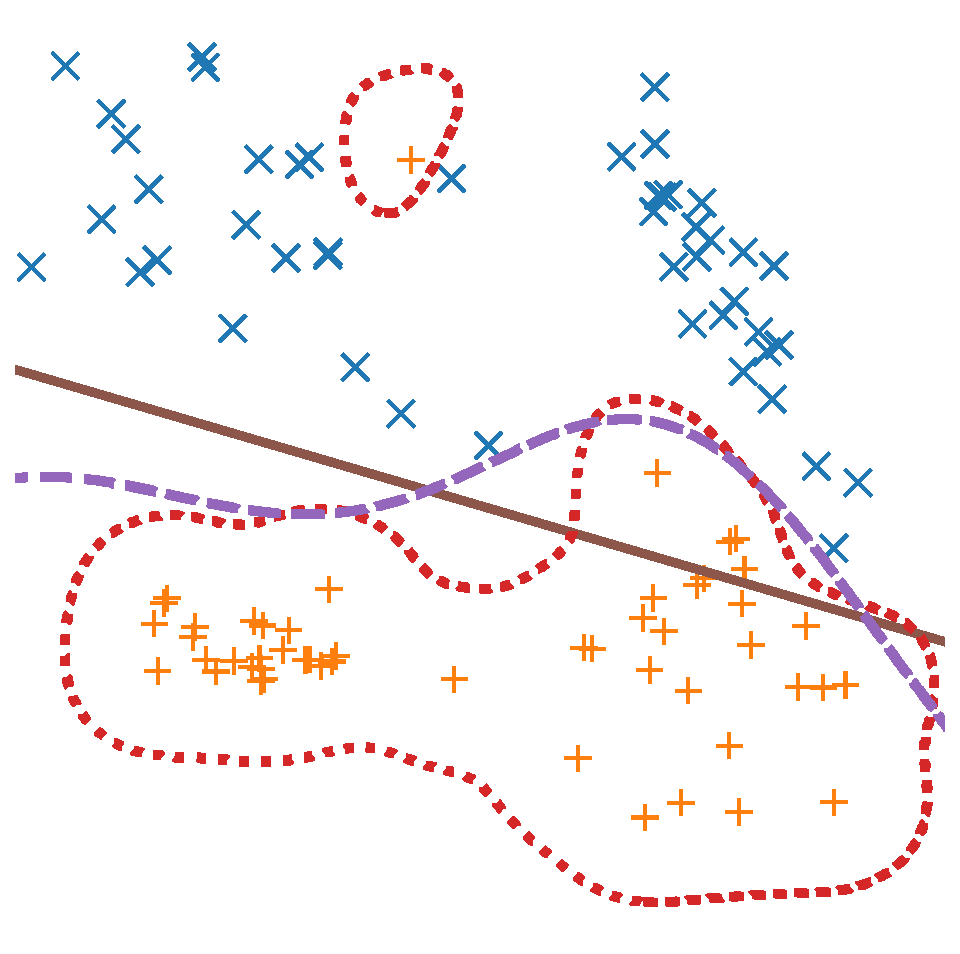
\includegraphics[width=\textwidth]{figures/generalisation/overfit_class}
    \caption{Pour séparer les observations négatives (x) des observations
      positives (+), la droite en trait plein sous-apprend. La frontière de
      séparation en pointillés ne fait aucune erreur sur les données mais est
      susceptible de surapprendre. La frontière de séparation en trait
      discontinu est un bon compromis.}
    \label{fig:overfit_class}
  \end{subfigure}
  \hfill
  \begin{subfigure}[t]{0.48\textwidth}
    \centering
    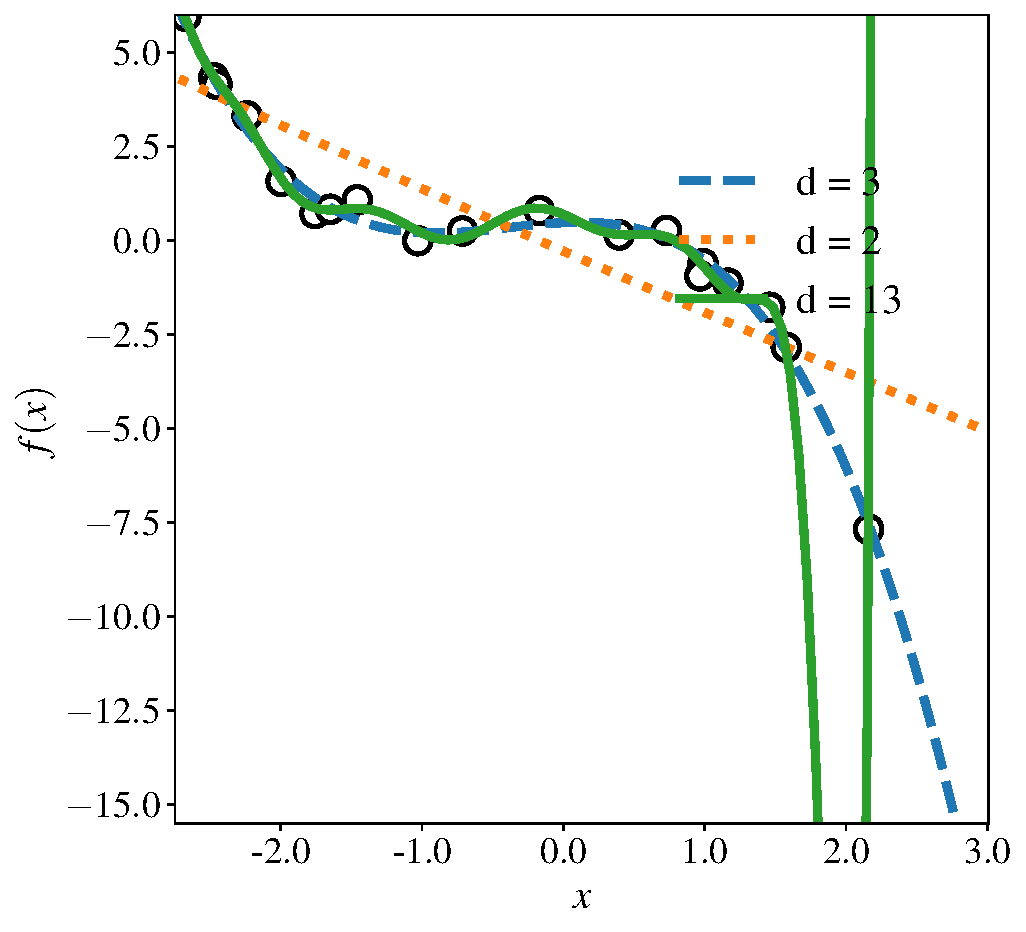
\includegraphics[width=\textwidth]{figures/generalisation/overfit_regr}
    \caption{Les étiquettes $y$ des observations (représentées par des points)
      ont été générées à partir d'un polynôme de degré $d=3$. Le modèle de
      degré $d=2$ approxime très mal les données et sous-apprend, tandis que
      celui de degré $d=13$, dont le risque empirique est plus faible,
      surapprend.}
    \label{fig:overfit_regr}
  \end{subfigure}
  \caption{Sous-apprentissage et surapprentissage}
\end{figure}

\subsection{Compromis biais-variance $\bullet$}
\label{sec:bias_variance}
Supposons disposer d'un jeu de données $\DD = \{\xx^i, y^i\}_{i=1, \dots, n}$
de $n$ observations en $p$ dimensions et leurs étiquettes réelles. Nous
supposons comme au chapitre précédent que les couples $(\xx^i, y^i)$ sont les
réalisations de $n$ vecteurs aléatoires de même loi qu'un couple de variables
aléatoire $(X, Y)$, $X$ étant un vecteur aléatoire $p$-dimensionnel et $Y$ une
variable aléatoire réelle à valeurs dans $\YY$, et qu'il existe une fonction
$\Phi \colon \RR^p \to \YY$ et une variable aléatoire réelle $\epsilon$
telle que
  \begin{equation}
  Y = \Phi(X) + \epsilon.
\end{equation}
Nous supposons de plus que $\epsilon$ est d'espérance nulle et de variance
$\sigma^2$.

Fixons maintenant un couple $(\xx, y) \in \RR^p \times \YY$. Nous pouvons
considérer que la prédiction $f(\xx)$ d'un modèle $f$ appris sur $\DD$ est une
estimation de $\Phi(\xx)$, autrement dit la réalisation d'une variable aléatoire
$F_n$ qui est une fonction d'un échantillon aléatoire de $n$ copies iid de
$(X, Y)$. Nous pouvons alors calculer l'erreur quadratique moyenne de la
prédiction $F_n$ :
\begin{align*}
  & \EE\left((y-F_n)^2\right)  = \EE\left((\Phi(\xx) + \epsilon - F_n)^2   \right)
   = \EE\left((\Phi(\xx) - \EE(F_n) + \EE(F_n) - F_n  + \epsilon )^2   \right) \\
  & = \EE\left((\Phi(\xx) - \EE(F_n))^2 + (\EE(F_n) - F_n  + \epsilon )^2 + 2
    (\Phi(\xx) - \EE(F_n))(\EE(F_n) - F_n  + \epsilon) \right) \\
  & = (\Phi(\xx) - \EE(F_n))^2 + \EE\left((F_n - \EE(F_n) - \epsilon )^2  \right) + 2
    (\Phi(\xx) - \EE(F_n))  \EE\left( \EE(F_n) - F_n  + \epsilon \right) \\
  & =  \text{B}(F_n)^2  + 
    \EE \left((F_n - \EE(F_n))^2 + \epsilon^2 - 2 \epsilon (F_n - \EE(F_n)) \right) + 2
    (\Phi(\xx) - \EE(F_n))  \left( \EE(F_n) - \EE(F_n)  + \EE(\epsilon) \right) \\
  & =  \text{B}(F_n)^2  + 
    \EE \left((F_n - \EE(F_n))^2 \right) + \EE(\epsilon^2) - 2 \EE\left(\epsilon (F_n - \EE(F_n)) \right) \\
    & = \text{B}(F_n)^2 + \VV(F_n) + \sigma^2.
\end{align*}
Le passage de la deuxième à la troisième ligne se fait par linéarité de
l'espérance et en observant que $\Phi(\xx)$ et $\EE(F_n)$ sont déterministes
(ce sont des nombres, pas des variables aléatoires).

Le troisième terme de la somme de la quatrième ligne disparait à la cinquième
car $\EE(\epsilon)=0$.

Enfin, le passage à la dernière ligne se fait en supposant que $\epsilon$ et
$F_n$ sont indépendants ; on a alors
$\EE\left(\epsilon (F_n - \EE(F_n)) \right) = \EE(\epsilon) \EE(F_n -
\EE(F_n)).$ De plus, $\EE(\epsilon^2) = \VV(\epsilon)$ car $\EE(\epsilon)=0$.

Ainsi, l'erreur quadratique moyenne est la somme
\begin{itemize}
\item du carré du biais de l'estimateur, qui quantifie à quel point les étiquettes prédites diffèrent des vraies étiquettes ;
\item de la variance de l'estimateur, qui quantifie à quel point les étiquettes
  prédites pour le même individu $\xx$ diffèrent selon les données d'entrée
  (i.e. les réalisations des n copies iid de $(X, Y)$) ;
\item de la variance du bruit, aussi appelée \textbf{erreur irréductible} : ce terme sera là même si l'estimation de $\Phi$ est exacte.
\end{itemize}

On retrouve ici le compromis biais-variance (cf
section~\ref{sec:precision_estimateur}) : un modèle biaisé peut, s'il a une variance plus faible, faire de meilleures prédictions qu'un modèle non-biaisé.



%Pour mieux comprendre le risque d'un modèle $f: \XX \rightarrow \YY$, nous
% pouvons le comparer à l'erreur minimale $\Rcal^*$ qui peut être atteinte par
% n'importe quelle fonction mesurable de $\XX$ dans $\YY$ : c'est ce qu'on
% appelle l'\textit{excès d'erreur}, et que l'on peut décomposer de la façon
% suivante :
% \begin{equation}
%   \label{eq:estimation_approximation}
%   \Rcal(f) - \Rcal^* = \left[ \Rcal(f) - \min_{h \in \FF} 
%     \Rcal(h) \right]
%   + \left[ \min_{h \in \FF} \Rcal(h) - \Rcal^* \right]
% \end{equation}

% Le premier terme, $\Rcal(f) - \min_{h \in \FF} \Rcal(h)$, quantifie la distance
% entre le modèle $f$ et le modèle optimal sur $\FF$. C'est ce que l'on appelle
% {\it l'erreur d'estimation.}

% Le second terme, $\min_{h \in \FF} \Rcal(h) - \Rcal^*$, quantifie la qualité du
% modèle optimal sur $\FF$, autrement dit, la qualité du choix de l'espace des
% hypothèses. C'est ce que l'on appelle {\it l'erreur d'approximation.} Si $\FF$
% est l'ensemble des fonctions mesurables, alors l'erreur d'approximation est
% nulle.

% Ainsi, l'écriture~\ref{eq:estimation_approximation} permet de décomposer
% l'erreur entre un terme qui découle de la qualité de l'espace des hypothèses et
% un autre qui découle de la qualité de la procédure d'optimisation utilisée. En
% pratique, sauf dans des cas très particuliers où cela est rendu possible par
% construction, il n'est pas possible de calculer ces termes d'erreur.
% Cependant, cette écriture nous permet de comprendre le problème suivant :
% choisir un espace des hypothèses plus large permet généralement de réduire
% l'erreur d'approximation, car un modèle plus proche de la réalité a plus de
% chances de se trouver dans cet espace. Cependant, puisque cet espace est plus
% vaste, la solution optimale y est aussi généralement plus difficile à trouver :
% l'erreur d'estimation, elle, augmente. C'est dans ce cas qu'il y a
% surapprentissage. \\

% Un espace des hypothèses plus large permet généralement de construire des
% modèles plus complexes : par exemple, l'ensemble des droites vs. l'ensemble des
% polynômes de degré 13 (cf. figure~\ref{fig:overfit_regr}). C'est une variante du
% principe du \textbf{rasoir d'Ockham}, selon lequel les
% hypothèses les plus simples sont les plus vraisemblables.

% Il y a donc un compromis entre erreur d'approximation et erreur d'estimation :
% il est difficile de réduire l'une sans augmenter l'autre. Ce compromis est
% généralement appelé \textbf{compromis biais-variance} : l'erreur d'approximation
% correspond au \textbf{biais} de la procédure d'apprentissage, tandis que l'erreur
% d'estimation correspond à sa \textbf{variance}. % On retrouvera ce compromis dans
% % l'estimation bayésienne de paramètres à la
% % section~\ref{sec:bias_variance_bayes}.

% Considérons par exemple pour un problème de régression un espace des hypothèses
% naïf qui ne contient que des fonctions constantes. Supposons que les étiquettes
% soient générées par une distribution normale centrée en $a$. Quelles que soient
% les données observées, la procédure d'apprentissage va construire un modèle qui
% retourne $a$ quelle que soit l'observation concernée : la \textbf{variance} de la
% procédure par rapport au jeu de données est très faible. À l'inverse, comme la
% fonction de prédiction apprise est très peu sensible au jeu de données, il y a
% un \textbf{biais} très important qui conduit à construire des prédicteurs qui
% retournent $a$ pour toutes les observations.

\section{Sélection de modèle}
Le théorème du \textit{no free lunch} % de~\citet{wolpert1997}
indique qu'aucun
algorithme de machine learning ne peut bien fonctionner pour \textbf{tous} les
problèmes d'apprentissage : un algorithme qui fonctionne bien sur un type
particulier de problèmes le compensera en fonctionnant moins bien sur d'autres
types de problèmes. En d'autres termes, il n'y a pas de \og baguette magique
\fg~qui puisse résoudre tous nos problèmes de machine learning, et il est donc
essentiel, pour un problème donné, de tester plusieurs possibilités afin de
sélectionner le modèle optimal. Notons au passage que plusieurs critères
peuvent intervenir dans ce choix : non seulement celui de la qualité des
prédictions, qui nous intéresse dans ce chapitre, mais aussi celui des
ressources de calcul nécessaires, qui peuvent être un facteur limitant en
pratique.

L'erreur empirique mesurée sur les observations qui ont permis de construire le
modèle est un mauvais estimateur de l'erreur du modèle sur l'ensemble des
données possibles, ou \textbf{erreur de généralisation} : si le modèle
surapprend, cette erreur empirique peut être proche de zéro voire nulle,
tandis que l'erreur de généralisation peut être arbitrairement grande.

\subsection{Jeu de test}
Il est donc indispensable d'utiliser pour évaluer un modèle des données
étiquetées qui n'ont pas servi à le construire. La manière la plus simple d'y
parvenir est de mettre de côté une partie des observations, réservées à
l'évaluation du modèle, et d'utiliser uniquement le reste des données pour le
construire.

Étant donné un jeu de données $\DD = \{(\xx^i, y^i)\}_{i=1, \dots, n}$,
partitionné en deux jeux $\DD_{\text{tr}}$ et $\DD_{\text{te}}$, on appelle
\textbf{jeu d'entraînement} (\textit{training set} en anglais) l'ensemble
$\DD_{\text{tr}}$ utilisé pour entraîner un modèle prédictif, et \textbf{jeu de
  test} (\textit{test set} en anglais) l'ensemble $\DD_{\text{te}}$ utilisé pour
son évaluation.

Comme nous n'avons pas utilisé le jeu de test pour entraîner notre modèle, il
peut être considéré comme un jeu de données \og nouvelles \fg. La perte
calculée sur ce jeu de test est un estimateur de l'erreur de généralisation.

Cela correspond à ce que nous avons fait dans la PC~3 et au début du Projet numérique.

\subsection{Jeu de validation}
Considérons maintenant la situation dans laquelle nous voulons choisir entre
$K$ modèles, appris chacun par un algorithme différent. Notons qu'il peut
s'agir ici d'utiliser des algorithmes d'apprentissage différents (plus proches
voisins, régression linéaire, réseau de neurones), ou d'un même algorithme
d'apprentissage avec plusieurs valeurs d'un ou plusieurs
\textbf{hyperparamètres}. Un hyperparamètre est un paramètre de l'algorithme
d'apprentissage (et non pas du modèle) ; il peut s'agir par exemple du nombre
de voisins $k$ considérés dans un algorithme des plus proches voisins (cf Projet numérique), du
coefficient de régularisation $\lambda$ dans un lasso (cf
section~\ref{sec:lasso}), ou du nombre de neurones dans une couche cachée d'un
perceptron multi-couche (cf section~\ref{sec:mlp}).

Nous pouvons alors entraîner chacun des modèles sur le jeu de
données d'entraînement, obtenant ainsi $K$ fonctions de décision
$f_1, f_2, \dots, f_K$, puis calculer l'erreur de chacun de ces modèles sur le
jeu de test. Nous pouvons ensuite choisir comme modèle celui qui a la plus
petite erreur sur le jeu de test:
\begin{equation}
  \hat f = \argmin_{k=1, \dots, K} \frac{1}{|\DD_{\text{te}}|} 
  \sum_{(\xx, y) \in \DD_{\text{te}}} L(y, f_k(\xx)).
\end{equation}
Mais quelle est son erreur de généralisation ? Comme nous avons utilisé
$\DD_{\text{te}}$ pour sélectionner le modèle, il ne représente plus un
jeu indépendant composé de données nouvelles, inutilisées pour déterminer le
modèle.

La solution est alors de découper notre jeu de données en \textbf{trois} parties~:
\begin{itemize}
\item Un \textbf{jeu d'entraînement}
  $\DD_{\text{tr}}$ sur lequel nous pourrons entraîner nos $K$ algorithmes
  d'apprentissage ;
\item Un \textbf{jeu de validation} ({\it validation set} en anglais)
  $\DD_{\text{val}}$ sur lequel nous évaluerons les $K$ modèles ainsi
  obtenus, afin de \textbf{sélectionner} un modèle définitif ;
\item Un \textbf{jeu de test} $\DD_{\text{te}}$ sur lequel nous évaluerons enfin
  l'erreur de généralisation du modèle choisi.
\end{itemize}

On voit ici qu'il est important de distinguer la {\it sélection} d'un modèle de
son \textbf{évaluation} : les faire sur les mêmes données peut nous conduire à
sous-estimer l'erreur de généralisation et le surapprentissage du modèle
choisi.

Une fois un modèle sélectionné, on peut le ré-entraîner sur l'union du jeu
d'entraînement et du jeu de validation afin de construire un modèle final.

\subsection{Validation croisée}
\label{sec:crossval}
La séparation d'un jeu de données en un jeu d'entraînement et un jeu de test
est nécessairement arbitraire. Nous risquons ainsi d'avoir, par hasard, créé
des jeux de données qui ne sont pas représentatifs. Pour éviter cet écueil, il
est souhaitable de reproduire plusieurs fois la procédure, puis de moyenner les
résultats obtenus afin de moyenner ces effets aléatoires. Le cadre le plus
classique pour ce faire est celui de la \textbf{validation croisée}, illustré sur
la figure~\ref{fig:crossval}

\begin{figure}[h]
  \centering
  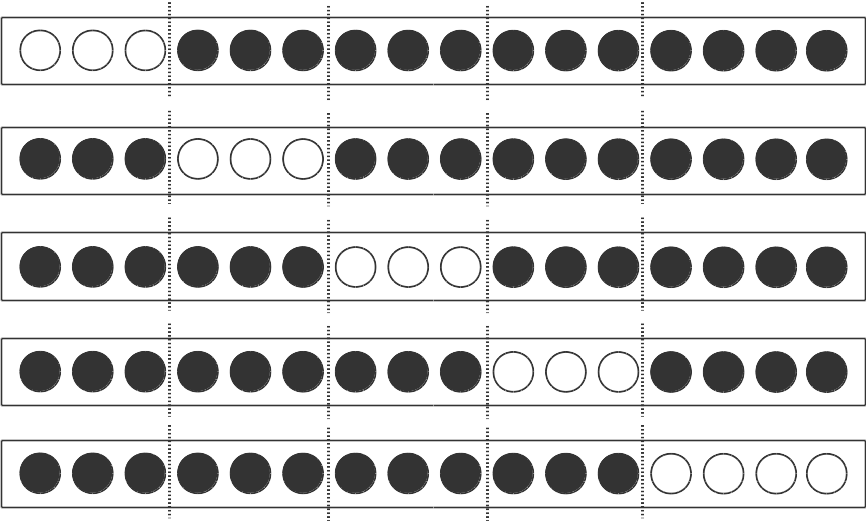
\includegraphics[width=0.5\textwidth]{figures/generalisation/crossval}
  \caption{Une validation croisée en 5 {\it folds} : Chaque observation
    appartient à un des 5 jeux de validation (en blanc) et aux 4 autres jeux
    d'entraînement (en noir).}
  \label{fig:crossval}
\end{figure}

Étant donné un jeu $\DD$ de $n$ observations, et un nombre $K$ (généralement
choisi égal à 5 ou 10), on appelle {\it validation croisée} la procédure qui
consiste à
\begin{enumerate}
\item partitionner $\DD$ en $K$ parties de tailles sensiblement similaires,
  $\DD_1, \DD_2, \dots, \DD_K$
\item pour chaque valeur de $k=1, \dots, K$,
  \begin{itemize}
  \item entraîner un modèle sur $\bigcup_{l \neq k} \DD_l$
  \item évaluer ce modèle sur $\DD_k$.
  \end{itemize}
\end{enumerate}
Chaque partition de $\DD$ en deux ensembles $\DD_k$ et $\bigcup_{l \neq
  k} \DD_l$ est appelée un \textbf{fold} de la validation croisée.

Chaque observation étiquetée du jeu $\DD$ appartient à un unique jeu de test,
et à $(K-1)$ jeux d'entraînement. Ainsi, cette procédure génère une prédiction
par observation de $\DD$. Pour conclure sur la performance du modèle, on évalue
chacun des $K$ prédicteurs sur le jeu de test $\DD_k$ correspondant, et on
moyenne ces performances. Cette approche permet aussi de rapporter l'écart-type
de ces performances, ce qui permet de se faire une meilleure idée de la
variabilité de la qualité des prédictions en fonction des données
d'entraînement.

\section{Critères de performance}
\subsection{Matrice de confusion et critères dérivés}
\label{sec:confusion_matrix}
Comme nous l'avons vu, le nombre d'erreurs de classification permet d'évaluer
la qualité d'un modèle prédictif. Notons que l'on préférera généralement
décrire le nombre d'erreurs comme une fraction du nombre d'exemples : un taux
d'erreur de $1\%$ est plus parlant qu'un nombre absolu d'erreurs.
 
Mais toutes les erreurs ne se valent pas nécessairement. Prenons l'exemple d'un
modèle qui prédise si oui ou non une radiographie présente une tumeur
inquiétante : une fausse alerte, qui sera ensuite infirmée par des examens
complémentaires, est moins problématique que de ne pas déceler la tumeur et de
ne pas traiter la personne concernée.  Les performances d'un modèle de
classification binaire peuvent être résumées dans une
\textbf{matrice de confusion} : une matrice $M$ de deux lignes et deux
colonnes, et dont l'entrée $M_{ck}$ est le nombre d'exemples de la classe $c$
pour laquelle l'étiquette $k$ a été prédite.
\begin{center}
  \begin{tabular}[h]{|c|c|c|c|} \hline \multicolumn{2}{|c}{} &
      \multicolumn{2}{|c|}{Classe réelle} \\ \hline \multicolumn{2}{|c|}{} & 0 & 1 \\ \hline 
    Classe & 0 & vrais négatifs (TN) & faux négatifs (FN)
    \\ \cline{2-4} prédite & 1 & faux positifs (FP) & vrais positifs (TP)
    \\ \hline
  \end{tabular}
\end{center}

% On retrouve ici les erreurs de première et de deuxième espèce de la
% section~\ref{sec:test_errors}, qu'on appellera plutôt respectivement faux
% positifs et faux négatifs dans ce contexte.

Il est possible de dériver de nombreux critères d'évaluation construits à
partir de la matrice de confusion, comme la spécificité, la sensibilité, le
rappel ou la F-mesure. Vous pouvez vous référer à la
section~\ref{sec:confusion_matrix_derived} à la fin de ce chapitre, ou à la
\href{https://scikit-learn.org/stable/modules/model_evaluation.html#classification-metrics}{documentation
  de \texttt{sklearn.metrics}}.



\subsection{Courbe ROC $\bullet$}
De nombreux algorithmes de classification ne retournent pas directement une
étiquette de classe, mais utilisent une fonction de décision qui doit ensuite
être seuillée pour devenir une étiquette. Cette fonction de décision peut être
un score arbitraire, ou la probabilité d'appartenir à la classe positive.
  
On appelle \textbf{courbe ROC}, de l'anglais \textbf{Receiver-Operator
  Characteristic} la courbe décrivant l'évolution de la sensibilité en fonction
du complémentaire à 1 de la spécificité, parfois appelé \textbf{antispécificité},
lorsque le seuil de décision change.

Le terme vient des télécommunications, où ces courbes servent à étudier si un
système arrive à séparer le signal du bruit de fond.

On peut synthétiser une courbe ROC par l'aire sous cette courbe, souvent
abrégée \textbf{AUROC} pour \textbf{Area Under the ROC}.

Un exemple de courbe ROC est présenté sur la figure~\ref{fig:roc_curve}. Le
point $(0, 0)$ apparaît quand on utilise comme seuil un nombre supérieur à la
plus grande valeur retournée par la fonction de décision : ainsi, tous les
exemples sont étiquetés négatifs. À l'inverse, le point $(1, 1)$ apparaît quand
on utilise pour seuil une valeur inférieure au plus petit score retourné par la
fonction de décision : tous les exemples sont alors étiquetés positifs.

\begin{figure}[h]
  \centering
  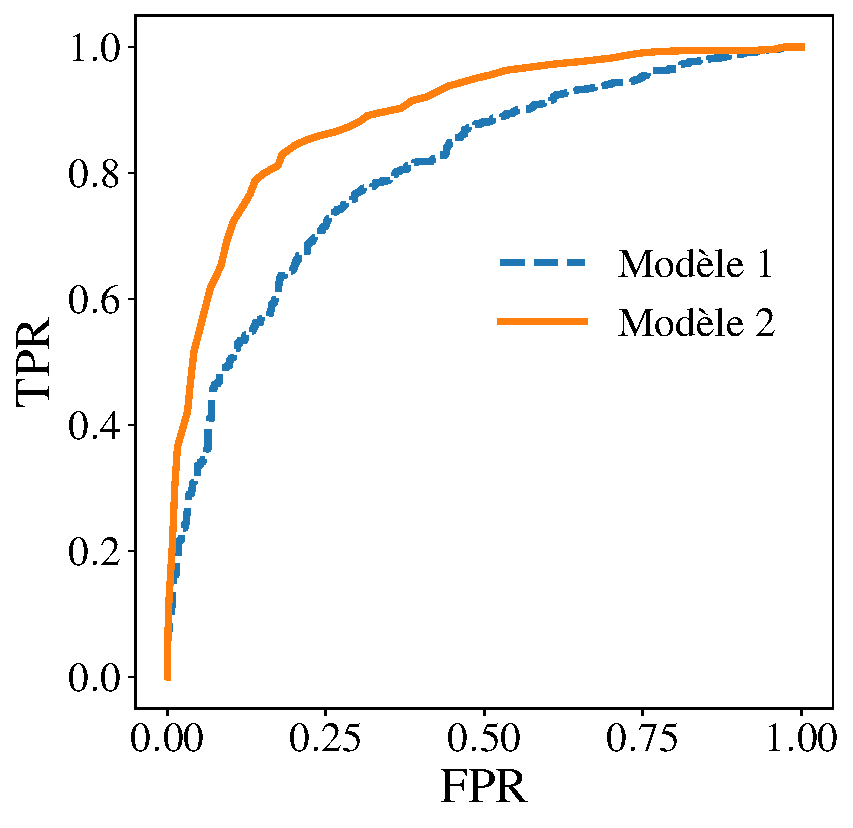
\includegraphics[width=0.5\textwidth]{figures/generalisation/roc_curve}
  \caption{Les courbes ROC de deux modèles.}
  \label{fig:roc_curve}
\end{figure}

Pour construire la courbe ROC, on prend pour seuil les valeurs successives de
la fonction de décision sur notre jeu de données. Ainsi, à chaque nouvelle
valeur de seuil, une observation que l'on prédisait précédemment négative
change d'étiquette. Si cette observation est effectivement positive, la
sensibilité augmente de $1/n_p$ (où $n_p$ est le nombre d'exemples positifs) ;
sinon, c'est l'antispécificité qui augmente de $1/n_n$, où $n_n$ est le nombre
d'exemples négatifs. La courbe ROC est donc une courbe en escaliers.

Un classifieur idéal, qui ne commet aucune erreur, associe systématique des
scores plus faibles aux exemples négatifs qu'aux exemples positifs. Sa courbe
ROC suit donc le coin supérieur gauche du carré $[0, 1]^2$ ; il a une aire sous
la courbe de 1.

La courbe ROC d'un classifieur aléatoire, qui fera sensiblement la même
proportion d'erreurs que de classifications correctes quel que soit le seuil
utilisé, suit la diagonale de ce carré. L'aire sous la courbe ROC d'un
classifieur aléatoire vaut donc 0.5.

On peut enfin utiliser la courbe ROC pour choisir un seuil de décision, à
partir de la sensibilité (ou de la spécificité) que l'on souhaite garantir.

\subsection{Erreurs de régression}
Un premier critère d'évaluation d'un modèle de régression est, nous l'avons vu
à plusieurs reprises, l'\textbf{erreur quadratique moyenne}, ou \textbf{MSE} de
l'anglais \textbf{mean squared error}, à savoir
\begin{equation*}
  \text{MSE} = \frac1n \sum_{i=1}^n \left( f(\xx^i) - y^i \right)^2.
\end{equation*}
Des variantes sont décrites dans la section~\ref{sec:regression_errors} ainsi que dans la \href{https://scikit-learn.org/stable/modules/model_evaluation.html#regression-metrics}{documentation de \texttt{sklearn.metrics}}.

\section{Régularisation}
\label{sec:generalization_regularization}
Le compromis biais-variance nous indique qu'un modèle biaisé peut être plus
précis qu'un modèle non-biaisé. La \textbf{régularisation} consiste ainsi à
ajouter au risque empirique que l'on cherche à minimiser un terme, appelé
\textbf{régulariseur}, qui va biaiser le modèle de sorte à ce que son risque
empirique soit plus élevée, mais son erreur de généralisation plus faible.

Plus un modèle est simple, et moins il a de chances de surapprendre. Pour
limiter le risque de surapprentissage, il est donc souhaitable de limiter la
complexité d'un modèle. Ainsi, le régulariseur peut être vu comme un terme qui
mesure la complexité du modèle. La définition de la complexité d'un modèle est
une notion importante en théorie de l'apprentissage, mais dépasse largement le
cadre de ce cours.

En appelant $\Omega$ le régulariseur, la régularisation consiste donc à
remplacer la minimisation du risque empirique (eq.~\eqref{eq:erm}) par :
\begin{equation}
  \label{eq:regularisation}
  f \in \argmin_{h \in \FF} \frac{1}{n} \sum_{i=1}^n L(y^i, h(\xx^i)) + 
  \lambda \Omega(h),
\end{equation}
où le \textbf{coefficient de régularisation} $\lambda \in \RR_+$ contrôle
l'importance relative de chacun des termes.


Quand $\lambda$ tend vers $+\infty$, le terme de régularisation prend de plus
en plus d'importance, jusqu'à ce qu'il domine le terme d'erreur et que seule
compte la minimisation du régulariseur : il n'y a plus d'apprentissage. % Dans la plupart des cas, le
% régulariseur est minimisé quand $\bbeta = \vec{0}$, et il n'y a plus
% d'apprentissage.
  
À l'inverse, quand $\lambda$ tend vers $0$, le terme de régularisation devient
négligeable devant le terme d'erreur, et la solution de
l'équation~\eqref{eq:regularisation} est un minimiseur du risque
empirique.% $\bbeta$ prendra comme valeur une
% solution de la régression linéaire non régularisée.

Comme tout hyperparamètre, $\lambda$ peut être choisi par validation
croisée. On utilisera généralement une grille de valeurs logarithmique.

La suite de cette section présente des exemples concrets de régularisation
appliquée à la régression linéaire. Nous reprenons les notations de la
section~\ref{sec:linreg}.


\section{Régularisation $\ell_2$  : régression ridge}
\label{sec:ridge_regression}
Une des formes les plus courantes de régularisation % , utilisée dans de
% nombreux domaines faisant intervenir des problèmes inverses mal posés,
consiste à utiliser comme régulariseur la norme $\ell_2$ du vecteur 
$\bbeta$ :  
\begin{equation}
  \label{eq:l2norm_reg}
  \Omega_{\text{ridge}}(\bbeta) = \ltwonorm{\bbeta}^2 = \sum_{j=0}^p \beta_j^2.
\end{equation}


On appelle \textbf{régression ridge} le modèle $f: x \mapsto \bbeta^\top \xx$ dont
les coefficients sont obtenus par
\begin{equation}
  \label{eq:ridgereg}
  \argmin_{\bbeta \in \RR^{p+1}} \ltwonorm{\yy - X \bbeta}^2 + 
  \lambda \; \ltwonorm{\bbeta}^2.
\end{equation}    

\paragraph{Solution}
Le problème~\eqref{eq:ridgereg} est un problème d'optimisation convexe : il s'agit de minimiser une forme
quadratique. Il se résout en annulant le gradient en $\bbeta$ de la fonction
objective :
\begin{equation}
  \nabla_{\bbeta} \left( \ltwonorm{\yy - X \bbeta}^2 + 
    \lambda \ltwonorm{\bbeta}^2 \right) = 0
\end{equation}

En notant $I_p \in \RR^{p \times p}$ la matrice identité en dimension $p,$ on
obtient :
\begin{equation}
  \left( \lambda I_p + X^\top X  \right) \bbeta^* = X^\top \yy.
\end{equation}
Comme $\lambda > 0$, la matrice $\lambda I_p + X^\top X$ est toujours
inversible. Notre problème admet donc toujours une unique solution
explicite. La régularisation par la norme $\ell_2$ a permis de transformer un
problème potentiellement mal posé en un problème bien posé, dont la solution
est :
\begin{equation}
  \label{eq:ridgereg_sol}
  \bbeta^* =  \left( \lambda I_p + X^\top X  \right)^{-1} X^\top \yy.
\end{equation}
  
% Si l'on multiplie la variable $x_j$ par une constante $\alpha$, le coefficient
% correspondant dans la régression linéaire non régularisée est divisé par
% $\alpha.$ En effet, si on appelle $X^*$ la matrice obtenue en remplaçant $x_j$
% par $\alpha x_j$ dans $X$, la solution $\bbeta^*$ de la régression linéaire
% correspondante vérifie $X^* \left( \yy - X^* \bbeta^* \right) = 0$, tandis que
% la solution $\bbeta$ de la régression linéaire sur $X$ vérifie
% $X \left( \yy - X \bbeta \right) = 0.$ Ainsi, changer l'échelle d'une variable
% a comme seul impact sur la régression linéaire non régularisée d'ajuster le
% coefficient correspondant de manière inversement proportionnelle.

% À l'inverse, dans le cas de la régression ridge, remplacer $x_j$ par
% $\alpha x_j$ affecte aussi le terme de régularisation, et a un effet plus
% complexe. L'échelle relative des différentes variables peut donc fortement
% affecter la régression ridge. Il est ainsi recommandé de \textbf{standardiser} les
% variables avant l'apprentissage, c'est-à-dire de toutes les ramener à avoir un
% écart-type de 1 en les divisant par leur écart-type :
% \begin{equation}
%   \label{eq:standardisation}
%   x_j^i \leftarrow \frac{x_j^i}{\sqrt{\frac1n \sum_{i=1}^n \left( x_j^i - 
%         \frac1n \sum_{i=1}^n x_j^i \right)^2}}
% \end{equation}    
% Attention : pour éviter le surapprentissage, il est important que cet
% écart-type soit calculé sur le jeu d'entraînement uniquement, puis appliqué
% ensuite aux jeux de test ou validation.

% La régression ridge a un effet de \og regroupement \fg~sur les variables
% corrélées, au sens où des variables corrélées auront des coefficients
% similaires.

\paragraph{Chemin de régularisation}
On appelle \textbf{chemin de régularisation} l'évolution de la valeur du
coefficient de régression d'une variable en fonction du coefficient de
régularisation $\lambda$.

Le chemin de régularisation permet de comprendre l'effet de la régularisation
sur les valeurs de $\bbeta$. En voici un exemple sur la
figure~\ref{fig:ridge_path}.

\begin{figure}[h]
  \centering
  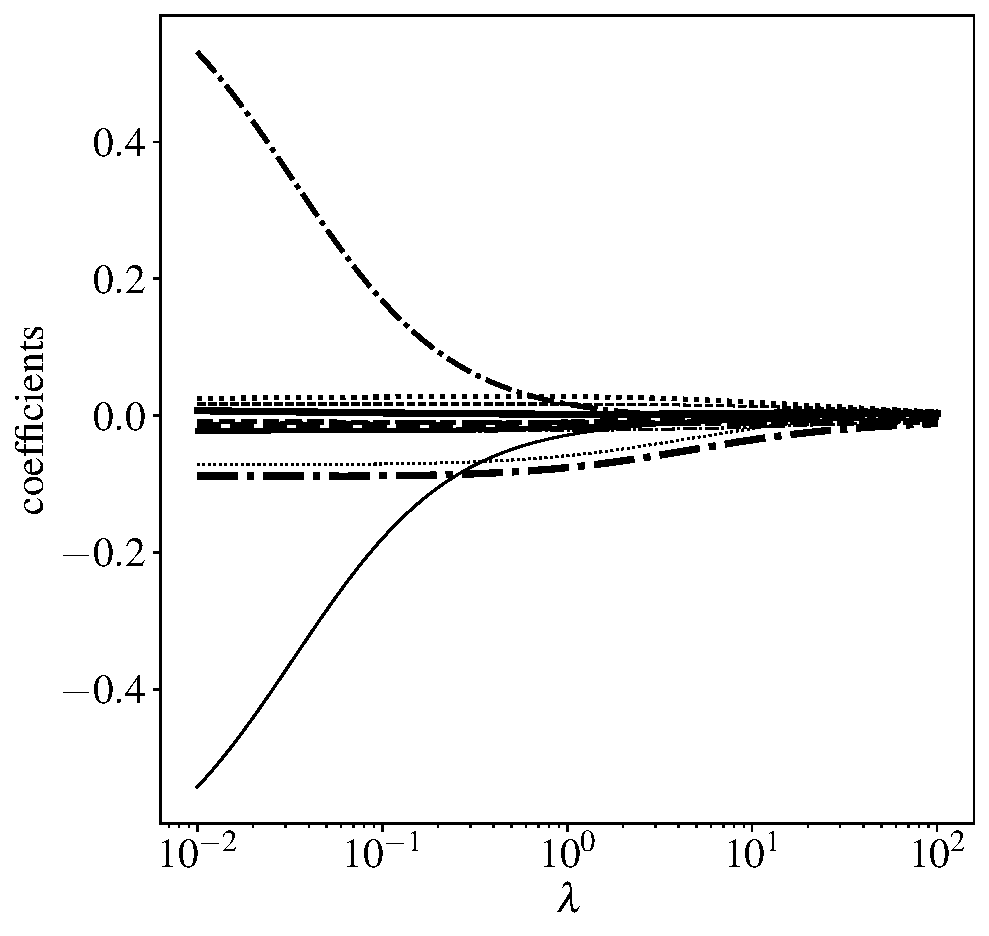
\includegraphics[width=0.5\textwidth]{figures/generalisation/ridge_path}
  \caption{Chemin de régularisation de la régression ridge pour un jeu de
    données avec 12 variables. Chaque ligne représente l'évolution du
    coefficient de régression d'une de ces variables quand $\lambda$ augmente :
    le coefficient évolue de sa valeur dans la régression non régularisée vers
    0.}
  \label{fig:ridge_path}
\end{figure}

\paragraph{Interprétation géométrique}
Étant donnés $\lambda \in \RR_+$, $X \in \RRnp$ et $\yy \in \RR^n$,
il existe un unique $t \in \RR_+$ tel que le problème~\eqref{eq:ridgereg} soit
équivalent à
\begin{equation}
  \label{eq:ridgereg_dual}
  \argmin_{\bbeta \in \RR^{p+1}} \ltwonorm{\yy - X \bbeta}^2 \text{ tel que }
  \ltwonorm{\bbeta}^2 \leq t.
\end{equation}
Preuve : L'équivalence s'obtient par dualité et en écrivant les conditions de
Karun-Kush-Tucker.
  
La régression ridge peut donc être formulée comme un problème d'optimisation
quadratique (minimiser $\ltwonorm{\yy - X \bbeta}^2$) sous contraintes
($\ltwonorm{\bbeta}^2 \leq t$) : la solution doit être contenue dans la boule
$\ell_2$ de rayon $\sqrt{t}$. Sauf dans le cas où l'optimisation sans
contrainte vérifie déjà la condition, cette solution sera sur la frontière de
cette boule, comme illustré sur la figure~\ref{fig:l2reg}.

\begin{figure}[h]
  \centering
  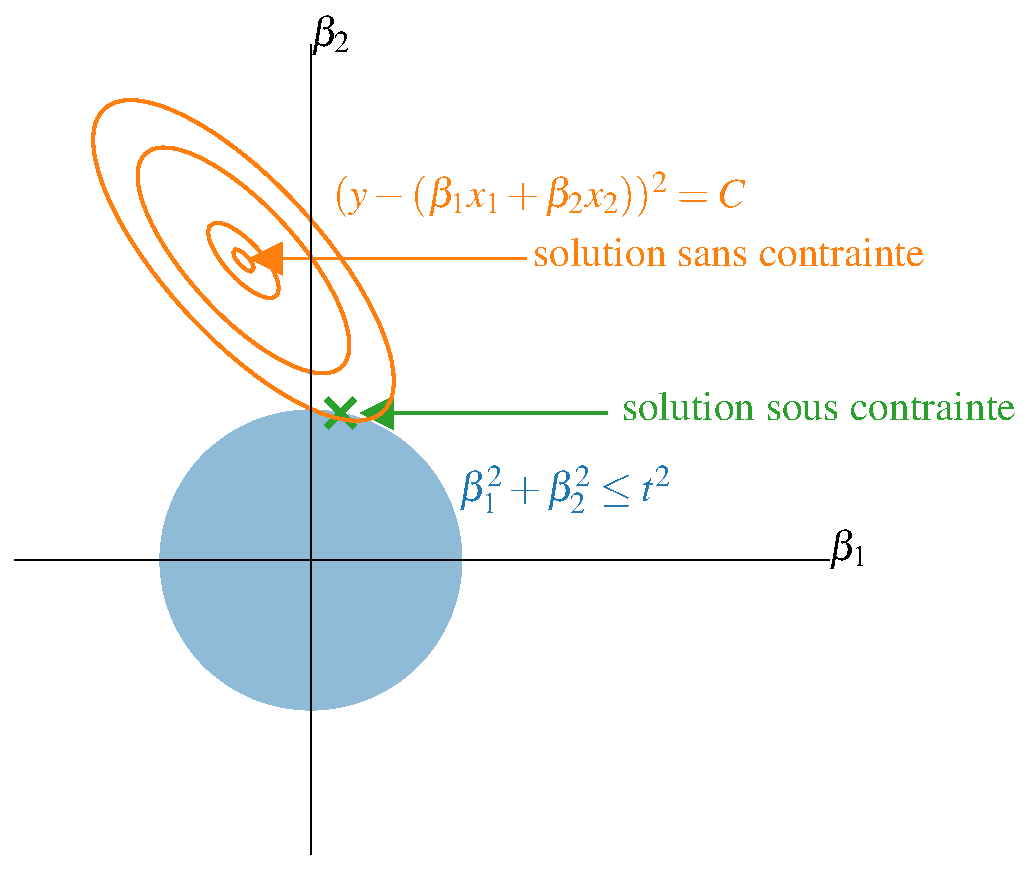
\includegraphics[width=0.55\textwidth]{figures/generalisation/l2reg}
  \caption{La solution du problème d'optimisation sous
    contraintes~\eqref{eq:ridgereg_dual} (ici en deux dimensions) se situe sur
    une ligne de niveau de la somme des moindres carrés tangente à la boule
    $\ell_2$ de rayon $\sqrt{t}$.}
  \label{fig:l2reg}
\end{figure}
  
\section{Régularisation $\ell_1$ : lasso}
\label{sec:lasso}

\paragraph{Parcimonie}
Dans certaines applications, il peut être raisonnable de supposer que
l'étiquette que l'on cherche à prédire n'est expliquée que par un nombre
restreint de variables. Il est dans ce cas souhaitable d'avoir un modèle {\it
  parcimonieux}, ou \textbf{sparse}, c'est-à-dire dans lequel un certain nombre de
coefficients sont nuls : les variables correspondantes peuvent être retirées du
modèle.

Pour ce faire, on peut utiliser comme
régulariseur la norme $\ell_1$ du coefficient $\bbeta$ :
\begin{equation}
  \label{eq:l1norm_reg}
  \Omega_{\text{lasso}}(\bbeta) = \lonenorm{\bbeta} = \sum_{j=0}^p \lvert \beta_j \rvert.
\end{equation}

On appelle \textbf{lasso} le modèle $f: x \mapsto \bbeta^\top \xx$ dont les
coefficients sont obtenus par
\begin{equation}
  \label{eq:lasso}
  \argmin_{\bbeta \in \RR^{p+1}} \ltwonorm{\yy - X \bbeta}^2 + 
  \lambda \lonenorm{\bbeta}.
\end{equation}    
Le nom de lasso est en fait un acronyme, pour \textbf{Least Absolute Shrinkage and
  Selection Operator} : il s'agit d'une méthode qui utilise les valeurs {\it
  absolues} des coefficients (la norme $\ell_1$) pour réduire (\textbf{shrink})
ces coefficients, ce qui permet de \textbf{sélectionner} les variables qui
n'auront pas un coefficient nul. En traitement du signal, le lasso est aussi
connu sous le nom de \textbf{poursuite de base} (\textbf{basis pursuit} en anglais).

En créant un modèle parcimonieux et en permettant d'éliminer les variables
ayant un coefficient nul, le lasso est une méthode de sélection de variables
supervisée. Il s'agit donc aussi d'une méthode de réduction de dimension.

\paragraph{Solution}
Le lasso~\ref{eq:lasso} n'admet pas de solution explicite. On pourra utiliser
un algorithme à directions de descente  pour le résoudre. De plus, il ne s'agit pas
toujours d'un problème strictement convexe (en particulier, quand $p > n$) et
il n'admet donc pas nécessairement une unique solution. En pratique, cela pose
surtout problème quand les variables ne peuvent pas être considérées comme les
réalisations de lois de probabilité continues.
Néanmoins, % s'il est possible que plusieurs $\bbeta$ minimisent la
  % fonction objective du lasso, leur produit à gauche par $X$ vaut toujours la
  % même valeur (par convexité stricte de la fonction de coût) ; cela permet de
  % montrer que 
il est possible de montrer que les coefficients non nuls dans deux solutions
ont nécessairement le même signe. Ainsi, l'effet d'une variable a la même
direction dans toutes les solutions qui la considèrent, ce qui facilite
l'interprétation d'un modèle appris par le lasso.
  
\paragraph{Interprétation géométrique}
Comme précédemment, le problème~\ref{eq:lasso} peut être reformulé comme un
problème d'optimisation quadratique sous contraintes :

Étant donnés $\lambda \in \RR_+$, $X \in \RRnp$ et $\yy \in \RR^n$,
il existe un unique $t \in \RR_+$ tel que le problème~\ref{eq:lasso} soit
équivalent à
\begin{equation}
  \label{eq:lasso_dual}
  \argmin_{\bbeta \in \RR^{p+1}} \ltwonorm{\yy - X \bbeta}^2 \text{ tel que }
  \lonenorm{\bbeta} \leq t.
\end{equation}

La solution doit maintenant être contenue dans la boule $\ell_1$ de rayon
$t$. Comme cette boule a des \og coins \fg, les lignes de niveau de la forme
quadratique sont plus susceptibles d'y être tangentes en un point où une ou
plusieurs coordonnées sont nulles (voir figure~\ref{fig:l1reg}).

\begin{figure}[h]
  \centering 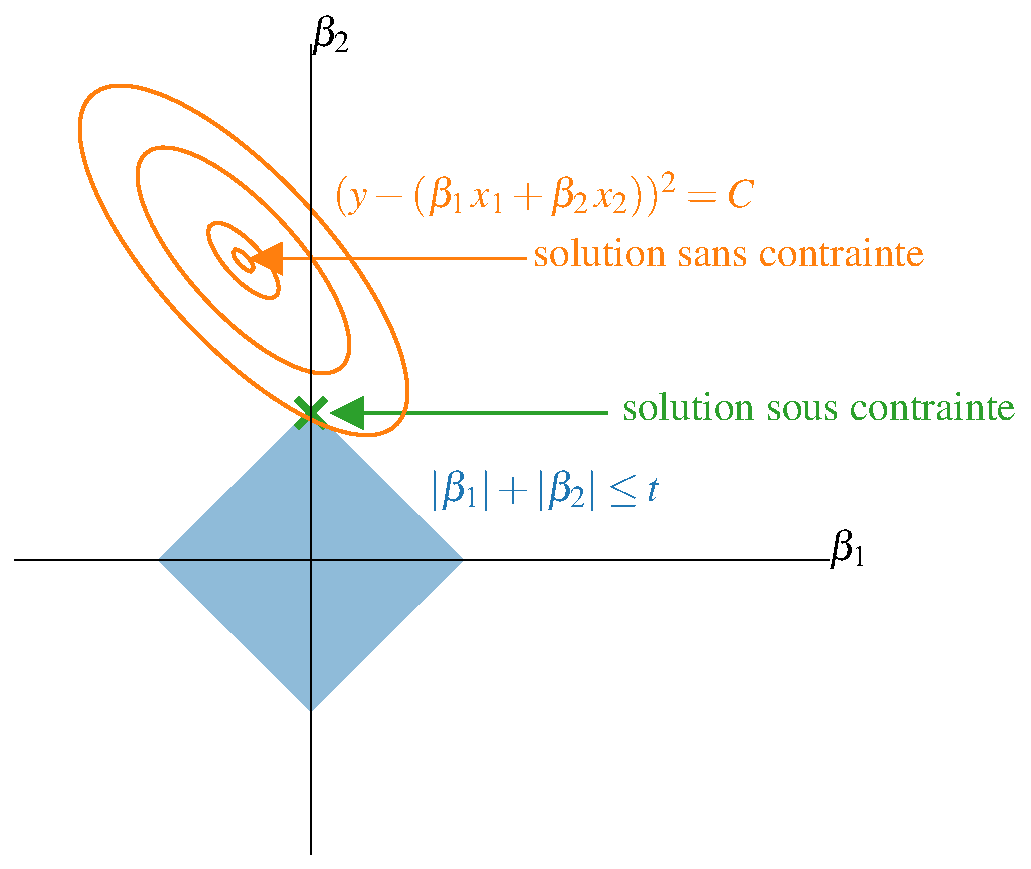
\includegraphics[width=0.55\textwidth]{figures/generalisation/l1reg}
  \caption{La solution du problème d'optimisation sous
    contraintes~\ref{eq:lasso_dual} (ici en deux dimensions) se situe sur
    une ligne de niveau de la somme des moindres carrés tangente à la boule
    $\ell_1$ de rayon $t$.}
  \label{fig:l1reg}
\end{figure}


\paragraph{Chemin de régularisation}
Sur le chemin de régularisation du lasso (par exemple
figure~\ref{fig:lasso_path}, sur les mêmes données que pour la
figure~\ref{fig:ridge_path}), on observe que les variables sortent du modèle
les unes après les autres, jusqu'à ce que tous les coefficients soient nuls. On
remarquera aussi que le chemin de régularisation pour n'importe quelle variable
est linéaire par morceaux ; c'est une propriété du lasso.
\begin{figure}[h]
  \centering
  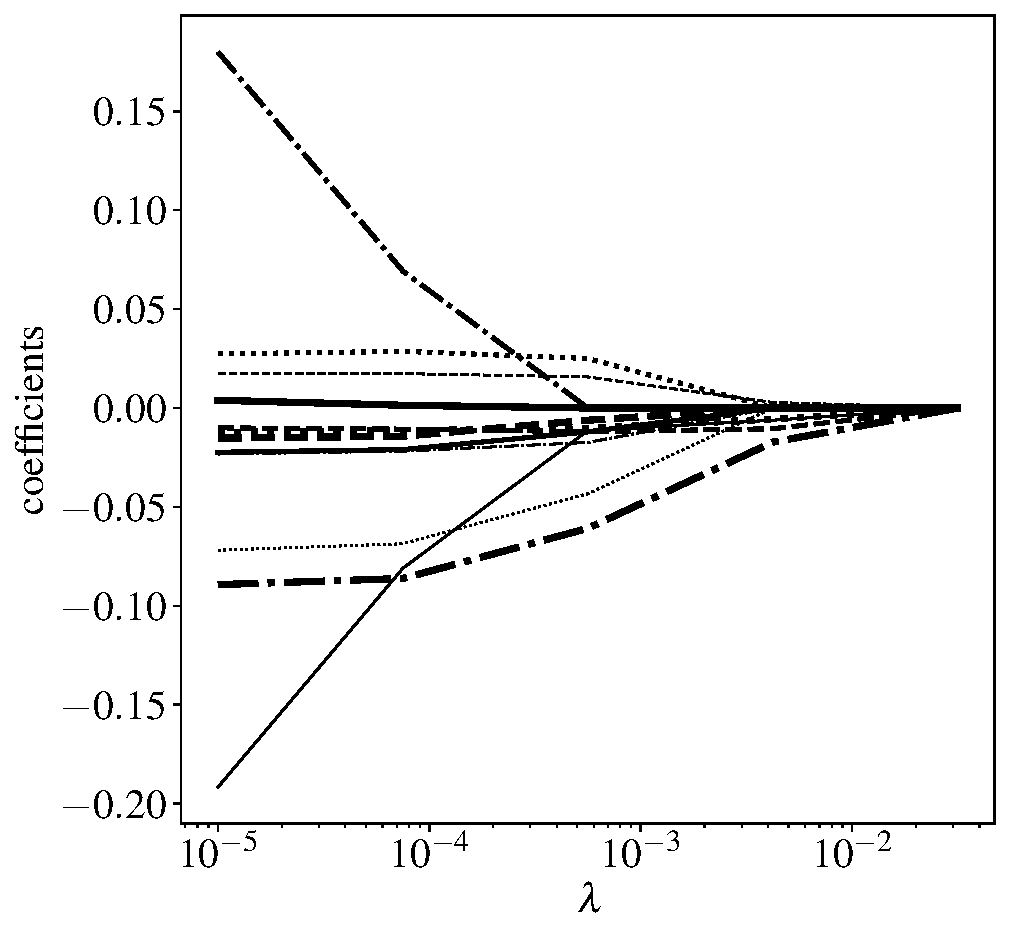
\includegraphics[width=0.5\textwidth]{figures/generalisation/lasso_path}
  \caption{Chemin de régularisation du lasso pour un jeu de données avec 12
    variables. Chaque ligne représente l'évolution du coefficient de régression
    d'une de ces variables quand $\lambda$ augmente : les variables sont
    éliminées les unes après les autres.}
  \label{fig:lasso_path}
\end{figure}

Si plusieurs variables corrélées contribuent à la prédiction de l'étiquette, le
lasso va avoir tendance à choisir une seule d'entre elles (affectant un poids
de 0 aux autres), plutôt que de répartir les poids équitablement comme la
régression ridge. C'est ainsi qu'on arrive à avoir des modèles très
parcimonieux. Cependant, le choix de cette variable est aléatoire, et peut
changer si l'on répète la procédure d'optimisation. Le lasso a donc tendance à
être instable.

% \section{Exercice : SVM linéaire pour la régression}
% \todo{}

\section{Compléments}
\subsection{Critères d'évaluation d'un modèle de classification binaire dérivés de la matrice de confusion}
\label{sec:confusion_matrix_derived}

On appelle \textbf{vrais positifs} (en anglais \textit{true positives}) les
exemples positifs correctement classifiés ; \textbf{faux positifs} (en anglais
\textit{false positives}) les exemples négatifs étiquetés positifs par le
modèle ; et réciproquement pour les \textbf{vrais négatifs} (\textit{true
  negatives}) et les \textbf{faux négatifs} (\textit{false negatives}). On note
généralement par \textbf{TP} le nombre de vrais positifs, \textbf{FP} le nombre
de faux positifs, \textbf{TN} le nombre de vrais négatifs et \textbf{FN} le
nombre de faux négatifs.

Il est possible de dériver de nombreux critères d'évaluation à partir de la
matrice de confusion. En voici quelques exemples :

On appelle \textbf{rappel} (\textbf{recall} en anglais), ou \textbf{sensibilité} ({\it
  sensitivity} en anglais), le taux de vrais positifs, c'est-à-dire la
proportion d'exemples positifs correctement identifiés comme tels :
\begin{equation*}
  \text{Rappel} = \frac{\text{TP}}{\text{TP} + \text{FN}}.
\end{equation*}

Il est cependant très facile d'avoir un bon rappel en prédisant que \textbf{tous}
les exemples sont positifs. Ainsi, ce critère ne peut pas être utilisé seul. On
lui adjoint ainsi souvent la \textbf{précision} :

On appelle \textbf{précision}, ou \textbf{valeur positive prédictive} (\textbf{positive
  predictive value, PPV}) la proportion de prédictions correctes parmi les
prédictions positives :
\begin{equation*}
  \text{Précision} = \frac{\text{TP}}{\text{TP} + \text{FP}}.
\end{equation*}

De même que l'on peut facilement avoir un très bon rappel au détriment de la
précision, il est aisé d'obtenir une bonne précision (au détriment du rappel)
en faisant très peu de prédictions positives (ce qui réduit le risque qu'elles
soient erronées)

L'anglais distingue \textbf{precision} (la précision ci-dessus) et \textbf{accuracy},
qui est la proportion d'exemples correctement étiquetés, soit le complémentaire
à 1 du taux d'erreur, aussi traduit par \textbf{précision} en français. On
utilisera donc ces termes avec précaution.

Pour résumer rappel et précision en un seul nombre, on calculera la
\textbf{F-mesure} (\textit{F-score} ou \textit{F1-score} en anglais), qui est
la moyenne harmonique de la précision et du rappel :
\begin{equation*}
  F = 2 \frac{\text{Précision . Rappel}}{\text{Précision} + \text{Rappel}} = 
  \frac{2 \text{TP}}{2 \text{TP} + \text{FP} + \text{FN}}.
\end{equation*}

Enfin, on appelle \textbf{spécificité} le taux de vrais négatifs, autrement dit la
proportion d'exemples négatifs correctement identifiés comme tels.
\begin{equation*}
  \text{Spécificité} = \frac{\text{TN}}{\text{FP} + \text{TN}}.
\end{equation*}

\subsection{Erreurs de régression}
\label{sec:regression_errors}
Pour mesurer l'erreur dans la même unité que celle des étiquettes, on préfère
souvent à l'erreur quadratique moyenne sa racine, généralement appelée
\textbf{RMSE} de l'anglais \textbf{root mean squared error} :

\begin{equation*}
  \text{RMSE} = \sqrt{\frac1n \sum_{i=1}^n \left( f(\xx^i) - y^i \right)^2}.
\end{equation*}

L'interprétation de la RMSE requiert néanmoins de connaître la distribution
des valeurs cibles : une RMSE de 1 cm n'aura pas la même signification selon
qu'on essaie de prédire la taille d'humains ou celle de drosophiles.  Pour
répondre à cela, il est possible de normaliser la somme des carrés des résidus
non pas en en faisant la moyenne, mais en la comparant à la somme des distances
des valeurs cibles à leur moyenne.  On appelle \textbf{erreur carrée relative},
ou \textbf{RSE} de l'anglais \textbf{relative squared error} la valeur
\begin{equation*}
  \text{RSE} = \frac{ \sum_{i=1}^n \left( f(\xx^i) - y^i \right)^2}{
    \sum_{i=1}^n \left( y^i - \frac1n \sum_{l=1}^n y^l \right)^2}.
\end{equation*}

Le complémentaire à 1 de la RSE est le \textbf{coefficient de détermination}, noté
$R^2$.

On note le coefficient de détermination $R^2$ car il s'agit du carré du
coefficient de corrélation de Pearson entre les prédictions et les valeurs réelles. 




\begin{plusloin}
\item Pour aller plus loin dans l'interprétation géométrique de la
  régularisation $\ell_1$ vs $\ell_2$, vous pouvez vous référer à l'animation
  sur
  \href{https://github.com/ievron/RegularizationAnimation/}{https://github.com/ievron/RegularizationAnimation/}
\item Une autre façon de voir la régularisation est de considérer qu'il s'agit
  d'utiliser un \textit{a priori} sur les coefficients du modèle. Ainsi, là où,
  pour la régression linéaire, la minimisation du risque empirique est
  équivalente à l'estimation par maximum de vraisemblance, la minimisation du
  risque empirique régularisé par la norme $\ell_2$ est équivalente à
  l'estimation par maximum \textit{a posteriori} avec un \textit{a priori} gaussien sur les
  coefficients du modèle. De même, la minimisation du risque empirique régularisé par
  la norme $\ell_1$ est équivalente à l'estimation  par maximum \textit{a posteriori} avec un \textit{a
    priori} suivant une distribution de Laplace. Pour plus de détails, on se
  rapportera au Chapitre 7 de
  \href{https://probml.github.io/pml-book/book0.html}{\textit{Machine Learning:
      A Probabilistic Perspective} de Kevin P. Murphy}
\item Au-delà des normes $\ell_1$ et $\ell_2$, il est possible d'utiliser des
  régulariseurs de la forme $\Omega_{\ell_q}(\bbeta) = ||\bbeta||_q^q.$
\item Une famille de régulariseurs appelés \og structurés \fg~permettent de
  sélectionner des variables qui respectent une structure (graphe, groupes, ou
  arbre) donnée a priori. Ces approches sont utilisées en particulier dans des
  applications bio-informatiques, par exemple quand on cherche à construire des
  modèles parcimonieux basés sur l'expression de gènes sous l'hypothèse que
  seul un petit nombre de voies métaboliques (groupes de gènes) est
  pertinent. Pour plus de détails, on se référera par exemple à
  \textit{Learning with structured sparsity}, J. Huang, T. Zhang \& D. Metaxas,
  Journal of Machine Learning Research 12:3371--3412 (2011).
\item Un ouvrage entièrement consacré au lasso et ses généralisations :
  \href{http://web.stanford.edu/~hastie/StatLearnSparsity/}{\textit{Statistical
      learning with sparsity: the {Lasso} and generalizations}}, T. Hastie,
  R. Tibshirani \& M. Wainwright (2015).
\item La régularisation est une technique importante des \textit{problèmes
    inverses} que vous pourrez découvrir dans l'ES du même nom l'an prochain. 
\end{plusloin}

%-*- coding: utf-8 -*-
\section{QCM}
\paragraph{Question 1.} Un modèle de régression régularisée est plus
  susceptible de surapprendre si le paramètre de régularisation est
\begin{itemize}
\item[$\square$] élevé ;
\item[$\square$] faible ;
\item[$\square$] ça dépend des cas.
\end{itemize}

\paragraph{Question 2.}     Dans un lasso, il y a plus de coefficients nuls quand le 
    paramètre de régularisation est 
\begin{itemize}
\item[$\square$] élevé ;
\item[$\square$] faible ;
\item[$\square$] ça dépend des cas.
\end{itemize}

\paragraph{Question 3.} Par rapport à un modèle complexe, un modèle plus simple est
\begin{itemize}
\item[$\square$] plus rapide à entraîner ;
\item[$\square$] plus susceptible de surapprendre ;
\item[$\square$] plus susceptible de bien généraliser ;
\item[$\square$] plus susceptible de minimiser le risque empirique.
\end{itemize}


\section*{Solution}
{%
\noindent
\rotatebox[origin=c]{180}{%
\noindent
\begin{minipage}[t]{\linewidth}
\paragraph{Question 1.}  Quand $\lambda$ est faible, c'est le risque empirique
qui domine et le modèle est plus susceptible de surapprendre. \newline

\paragraph{Question 2.} Quand $\lambda$ croît, le régulariseur prend plus
d'importance et le nombre de coefficients nuls augmente. \newline

\paragraph{Question 3.} Le temps d'entrainement ne dépend pas toujours de la
complexité du modèle. Un modèle plus simple sera cependant souvent plus
rapide à entrainer.

Un modèle simple est moins susceptible de surapprendre (et plus susceptible de sousapprendre) ; généralisera mieux, sauf s'il est en sous-apprentissage ; et minimisera moins bien le risque empirique.
\end{minipage}%
}%


%%% Local Variables:
%%% mode: latex
%%% TeX-master: "../../sdd_2025_poly"
%%% End:



%%% Local Variables:
%%% mode: latex
%%% TeX-master: "../sdd_2025_poly"
%%% End: